\documentclass[a4paper,10pt]{article}
\usepackage[top=1.8cm,bottom=1.8cm,left=1.8cm,right=1.8cm,asymmetric]{geometry}
\usepackage{url}
\usepackage{paralist}
\usepackage{authblk}
\usepackage{graphicx}
\usepackage[pdftex,colorlinks=true,hyperfootnotes=false]{hyperref}

\title{\vspace{-4em}A System for Automating Reproducibility in Science}

\author[1]{Tom Crick}
\author[2]{Benjamin A. Hall}
\author[3]{Samin Ishtiaq}
\affil[1]{Department of Computing \& Information Systems, Cardiff Metropolitan University}
\affil[2]{MRC Cancer Unit, University of Cambridge}
\affil[3]{Microsoft Research Cambridge}
\affil[1]{\protect\url{tcrick@cardiffmet.ac.uk}}
% \affil[2]{\protect\url{bh418@mrc-cu.cam.ac.uk}}
% \affil[3]{\protect\url{samin.ishtiaq@microsoft.com}}


\renewcommand\Authands{ and }
\def\UrlBreaks{\do\/\do-}

\date{ }

\begin{document}
\maketitle

\begin{abstract}
We propose a prototype open software platform on Azure which will
automate reproducibility for algorithms and models, linking together
research software and data repositories, toolchains, workflows and
outputs, providing a seamless infrastructure for the verification and
validation of scientific models and in particular, performance
benchmarks for a wide range of computational research disciplines.
\end{abstract}


%\vspace{-1.5cm}
\subsection*{Introduction}

Reproducibility (replication, repeatability) is a basic tenet of good
science. This tenet holds all the more for digital science, with its
fundamentally more concrete outputs of algorithms and models. However,
there remain cultural and technical barriers to the sharing (using,
repeating, comparing, contributing, reimplementing) of these
artefacts, all the way from disseminating academic publications
through to recognition of the importance of scientific software and
computation.

We believe that an automated notify+reproduce system built on Azure,
which allows easy reproduction of the results of algorithms running on
models, will help significantly with lifting the cultural burden and,
by doing so, will vastly improve the efficiency of scientific
exploration. This Microsoft Azure for Research grant application
builds on this belief. While there has been significant academic and
policy discussion in this space over the past few years, now is the
time for the creation of an extensible and adaptable open
infrastructure to facilitate the automation of science
reproducibility.


\subsection*{Description}
{\textbf{We propose to develop a prototype open software platform on
Azure which will automate reproducibility for algorithms and models.}}
By developing a cloud-based, centralised service, which performs
automated code compilation, testing and benchmarking (with associated
auditing), we will link together published implementations of
algorithms and input models. This will allow the prototype to link
together software and data repositories, toolchains, workflows and
outputs, providing a seamless automated infrastructure for the
verification and validation of scientific models and in particular,
performance benchmarks. The program of work will lead the cultural
shift in both the short and long-term to move to a world in which
computational reproducibility helps researchers achieve their goals,
rather than being perceived as an overhead.

A system as described here has several up-front benefits: it links
research papers more closely to their outputs, making external
validation easier and allows interested users to explore unaddressed
sets of models. Critically, it helps researchers across computational
science to be more productive, rather than reproducibility being an
overhead on their day-to-day work. In the same way that tools such as
GitHub make collaborating easier while simultaneously allowing
effortless sharing, we envisage our system being similarly usable for
sharing and testing algorithms, software, models and benchmarks
online.

While there are several web-based services that can do certain parts
of what our proposed system will do, it will be a significant
engineering task to create a service that can integrate all of these
features (as well as effect the required socio-cultural change within
the computational science community). However, such a service would
then allow algorithms and models to evolve together, and be
reproducible from the outset.

In summary, this proposed new infrastructure, previously presented and
discussed by the authors (in collaboration with Kenji Takeda of
Microsoft
Research\footnote{\url{http://blogs.msdn.com/b/msr_er/archive/2014/12/11/reproducibility-as-a-service-can-the-cloud-make-it-real.aspx}})~\cite{crick-et-al_wssspe2,crick-et-al_recomp2014},
would have a profound impact on the way that open computational
science is performed, repositioning the role of models, algorithms and
benchmarks and accelerating the research cycle. Furthermore, it would
effect the vital cultural change by reducing overheads and improving
the efficiency of researchers.

\subsection*{Vision}

In the software development world, no one would (or should!) commit to
a project without first running the smoke tests. You could be clever
and run the tests via the version control system's pre-commit
hook. That way you would never forget to run the tests. All of this
can be done, at scale, on the cloud now. Services such as Visual
Studio Online and Jenkins, etc, schedule the tests to run as soon as
you commit. We envisage moving to a world in which benchmarks become
available online, in the same vein as open access of publications and
research data. It seems an obvious step to hook these continuous
integration (CI) systems up to the algorithm implementations that are
written to run on these benchmarks.

Suppose you have come up with a better algorithm to deal with some of
these benchmarks. You write up the paper on the algorithm but, more
importantly, you also register the implementation of your algorithm at
this open service, as a possible algorithm to run on this benchmark
set. The benchmarks live in distributed git repositories. Some of the
servers that house these repositories are CI servers. Now, when you
push a commit to your algorithm, or someone else pushes a commit to
theirs, or when someone else adds a new benchmark, the service's CI
system is triggered. It is also activated with the addition of a new
library, firmware upgrade, API change, etc. All registered algorithms
are run on all registered models, and the results are published. The
CI servers act as an authoritative source (analogous to the Linux
Kernel Archives) of results for these algorithms running on these
benchmarks.

\subsection*{Workflow}

\begin{figure}[!h]
\centering
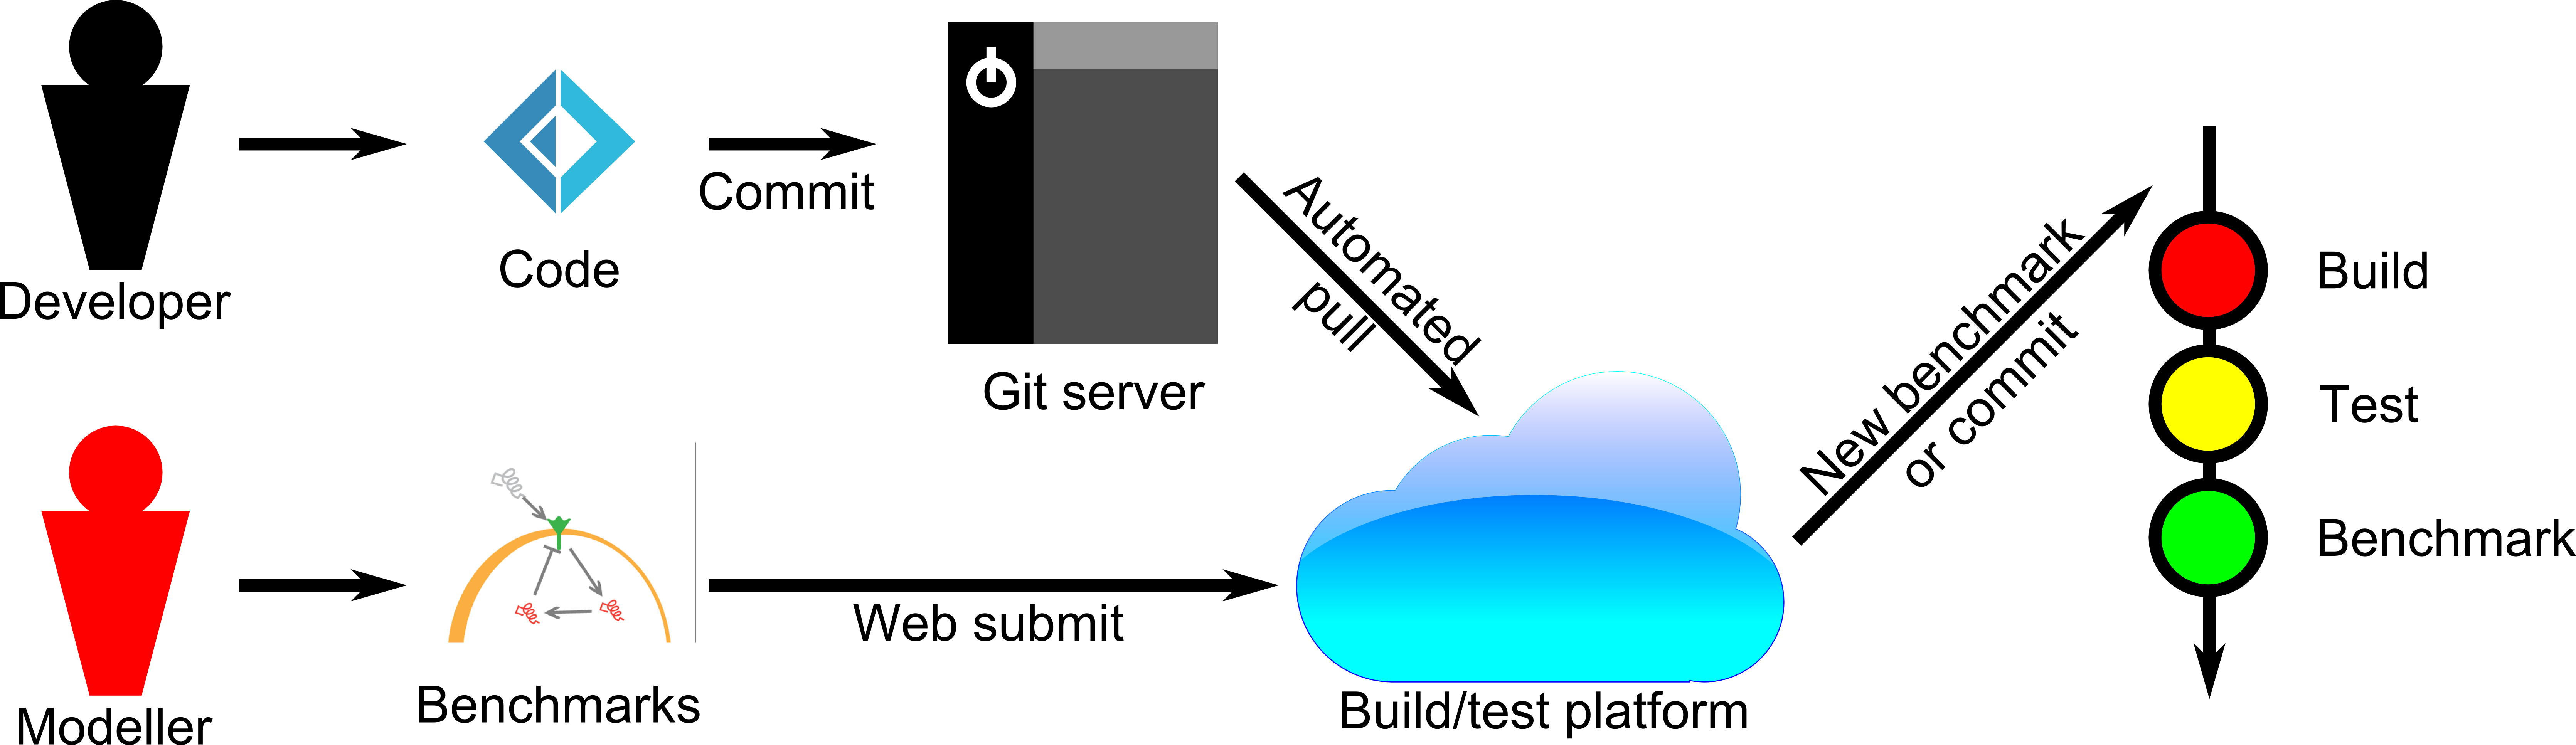
\includegraphics[width=\columnwidth]{workflow.png}
\caption{Proposed system workflow.}
\label{fig:workflow}
\end{figure}

The objective of this proposal is to develop a system (see
Figure~\ref{fig:workflow}) which, through integration with publicly
available source code repositories, automates the build, testing and
benchmarking of algorithms and benchmarks. The system will allow
testing models against competing algorithms, and the addition of new
models to the test suite (either manually or from existing online
repositories). The goals are thus to:\\

\begin{compactitem}
	\item Build a cloud service which automatically pulls and compiles
code from git repositories;
\item Run automated tests defined by the developers on the code;
\item Perform analysis of benchmark sets supplied by both the developer and external
users;
\item Provide persistent audit trails for software and benchmarks results;
\item Collaborate with key stakeholders in the open software/open data/open access/open
  science space, as well as key e-infrastructure organisations
  e.g. GitHub, figshare, Software Sustainability
  Institute, Mozilla Science Lab, Digital Science, etc.
\end{compactitem}

\subsection*{Resources}

For the Azure resources we require for our prototype, we have profiled
three project sizes: {\emph{small}}, {\emph{medium}} and
{\emph{large}}, estimating the required compute storage units per
``customer''. Under these assumptions, we would require spawning of
compute in burst mode (potentially scaling hundreds/thousands of hours
of compute time), with an appropriate amount of (scratch) storage for
the pull/compile/run process, along with a persistant extendible
database for auditing and tracking:\\

\begin{compactitem}
\item {\emph{small}}: project consisting of c.10,000 lines of code,
  c.10GB storage
\item {\emph{medium}}: project consisting of c.100,000 lines of code,
  c.25GB storage
\item {\emph{large}}: project consisting of c.1,000,000 lines of code,
 c.50GB storage\\
\end{compactitem}

An example of one of our target projects is Z3, a high-performance
theorem prover being developed at Microsoft
Research\footnote{\url{http://z3.codeplex.com/}}. Z3 is a
{\emph{medium}}-sized project requiring the spawning of four-core
compute VMs used overnight, with the associate storage and database
requirements as outlined above. Further target projects include the
Bio Model Analyzer\footnote{\url{http://biomodelanalyzer.research.microsoft.com/}},
a biological modelling tool that illustrates signalling pathways and
determines cellular stabilisation, as well as solver tools for logic
programming
e.g. Potassco\footnote{\url{http://potassco.sourceforge.net/}}, the
Potsdam Answer Set Solving Collection, all with similar or greater
computational requirements.

The system will be developed over a period of six months starting January
2015, including regular meetings (predominantly in Cambridge, UK) for
the design and requirements of the tool, and will involve the
employment of a dedicated programmer to implement the bulk of the
system (this has been costed under our shortlisted Digital
Science Catalyst
Grant\footnote{\url{http://www.digital-science.com/what-we-do/start-up-investment/catalyst}}
application, awaiting award decision in December 2014).

\subsection*{Dissemination and Impact}

The dissemination, wide usage and thus impact of our system is
critical. Between the project team, we have three discrete (and widely
applicable) application domains (theorem proving, biological modelling
and logic programming) ready and willing to provide pilot tests for
our system. We will also be working closely with the Software
Sustainability Institute (Crick is a 2014 Fellow) and associated
community, as well as with colleagues at
Recomputation.org\footnote{\url{http://recomputation.org}; also see
the Recomputation Manifesto: \url{http://arxiv.org/abs/1304.3674}},
the repository for experiments in computational science. Furthermore,
we intend on disseminating outcomes from this project in range of
appropriate high-impact conference and journals, with a paper
currently envisaged for
Toolbox\footnote{\url{http://www.nature.com/news/toolbox}}, Nature's
hub for scientific software, apps and online tools.

More generally, we will also collaborate with key stakeholders in the
open software/open data/open access/open science space, as well as key
e-infrastructure organisations e.g. GitHub, figshare, Mozilla Science
Lab, Digital Science, etc, to further showcase to the wider research
community.

\subsection*{Project Team}

Dr Tom Crick\footnote{\url{http://drtomcrick.com}} is a Senior Lecturer in
Computing Science at Cardiff Metropolitan University, having completed
his PhD and post-doctoral research at the University of Bath. His
research interests cut across computational science: knowledge
representation and reasoning, intelligent systems, big data analytics,
optimisation and high performance computing.  He is the Nesta Data
Science Fellow, a 2014 Fellow of the Software Sustainability Institute
(EPSRC) and a member of {\emph{HiPEAC}}, the European FP7 Network of
Excellence on High Performance and Embedded Architecture and
Compilation.

Dr Benjamin A. Hall\footnote{\url{http://www.mrc-cu.cam.ac.uk/hall.html}} is a
Royal Society University Research Fellow, developing hybrid and formal
models of carcinogenesis and biological signalling at the MRC Cancer
Unit, University of Cambridge. He previously worked at Microsoft
Research Cambridge (on BMA with Jasmine Fisher), UCL and the
University of Oxford. As part of his role at Oxford, he was one of two
Apple Laureates, awarded by Apple and the Oxford Supercomputing Centre
for the project {\emph{A biomolecular simulation pipeline}}. Benjamin
has an MBiochem and DPhil from the University of Oxford.

Dr Samin Ishtiaq\footnote{\url{http://research.microsoft.com/en-us/people/sishtiaq/}}
is Principal Engineer in the Programming Principles and Tools group at
Microsoft Research Cambridge. He currently works on the SLAyer
(Separation Logic-based memory safety for C programs), TERMINATOR
(program termination) and BMA projects. Samin joined MSR in April
2008. Before that (2000-2008), he worked in CPU modelling and
verification at ARM, helping to tape-out the Cortex A8, Cortex M3 and
SC300 processors, and the AMBA bus protocol checker. Samin has an MEng
from Imperial and a PhD in dependent type theory from Queen Mary.

\bibliographystyle{unsrt}
\bibliography{Azure4Research}

\end{document}
